%!TEX root = ../memoire.tex

\chapter{La génération automatique de texte}

%%%%%%%%%%%%%%%%%%%%%%%%%%%%%%%%%%%%%%%%%%%%%%%%%%%%%%%
% --------- I N T R O   ---------
%%%%%%%%%%%%%%%%%%%%%%%%%%%%%%%%%%%%%%%%%%%%%%%%%%%%%%%

La \acf{GAT} est une branche du \acf{TAL} à la croisée des chemins entre l'intelligence artificielle et la linguistique computationnelle \citep{ReiterBuildingNaturalLanguage2000}. L'objectif de la \ac{GAT} est de produire du texte compréhensible en langue naturelle à partir de données (non-linguistiques). Bien que cet objectif soit commun à tous les générateurs de texte, il existe diverses méthodes pour y arriver. La diversité des méthodes est une conséquence directe de la combinaison des divers types d'inputs possibles et des multiples approches de réalisation. Par exemple, les systèmes de \ac{GAT} peuvent prendre en input du texte, des données numériques et même des images \citep{thomason:coling14}.

Les premiers systèmes de \ac{GAT} ont été conçus pour générer des rapports automatiquement afin de faciliter le travail humain \citep{ReiterBuildingNaturalLanguage2000}. En effet, \cite{DaoustJSREALTextRealizer2015} soulignent dans leur article que la \ac{GAT} nous permet de générer un résumé d'information compréhensible pour un humain à partir de données brutes qui seraient normalement difficiles à lire. Ces tâches automatisées permettent d'éviter des coûts en termes de ressources et de temps. Autrement, la production de tels rapport est faite par un humain, ce qui entraîne des coûts importants souvent prohibitifs.

Les textes générés automatiquement n'ont pas besoin d'être lus par une grande quantité de gens pour être considérés utiles. On considèrera qu'ils remplissent leur fonction dès qu'ils comblent un besoin. De plus, les produits des systèmes de \ac{GAT} peuvent aussi être \emph{taillés sur mesure}, en fonction des besoins de l'utilisateur \citep{1948c0b7a8ca42679cad977bb2cdddc2}. Par exemple, le système MARQUIS a implémenté cette composante en permettant à des utilisateurs de recevoir des bulletins sur la qualité de l'air en fonction de leur santé ou de leur profession \citep{WannerMARQUISGENERATIONUSERTAILORED2010}.

D'autres chercheurs ont même poussé la \ac{GAT} vers le domaine journalistique qu'on dénomme le robo-journalisme. Concrètement, ces systèmes prennent en entrée des données brutes concernant un match donné et produisent un article qui en décrit le déroulement \citep{W17-3513}. En effet, il semble y avoir une demande pour cette branche de la \ac{GAT} puisqu'il y existe un grand nombre d'évènements qui ne sont pas couverts, mais qui pourraient intéresser des gens. Ce problème a également incité \citeauthor{dras12} à développer un système de \ac{GAT} produisant des descriptions de matchs de football australien en anglais et en arrernte (langue aborigène) \citep{lareau11a,dras12}: les aborigènes australiens adorent le football australien, mais peu de couverture médiatique existe dans leur langue.

Finalement, il est aussi important de préciser que la \ac{GAT} présente un intérêt pour la linguistique théorique. En effet, les linguistes peuvent s'en servir pour tester leurs théories et vérifier si leur modélisation de la langue contient des erreurs \citep{DanlosPresentationmodelegeneration1983}. 

%%%%%%%%%%%%%%%%%%%%%%%%%%%%%%%%%%%%%%%%%%%%%%%%%%%%%%%
% --------- P I P E L I N E   ---------
%%%%%%%%%%%%%%%%%%%%%%%%%%%%%%%%%%%%%%%%%%%%%%%%%%%%%%%

\section{Pipeline classique GAT} \label{ppc}

Selon \cite{ReiterBuildingNaturalLanguage2000}, un système de \ac{GAT} se découpe en six modules, que nous illustrons à la figure~\ref{fig:Pipeline}. De façon plus grossière, on peut séparer ces modules en deux étapes majeures: le \emph{quoi-dire} et le \emph{comment-le-dire} \citep{DanlosPresentationmodelegeneration1983}, qui correspondent aux \emph{early process} et \emph{late process} de \cite{gatt18}. Le \emph{quoi-dire} fait référence à la sélection du contenu, la structuration du document et l'agrégation. Puis le \emph{comment-le-dire} fait référence à toutes les étapes subséquentes: la lexicalisation, la génération d'expressions référentielles et la réalisation linguistique. Pour mieux comprendre ce processus séquentiel, nous décrirons en quelques lignes chacune des étapes qui le composent.

\begin{figure}[htb] % utilise toujours [htb]
	\centering
	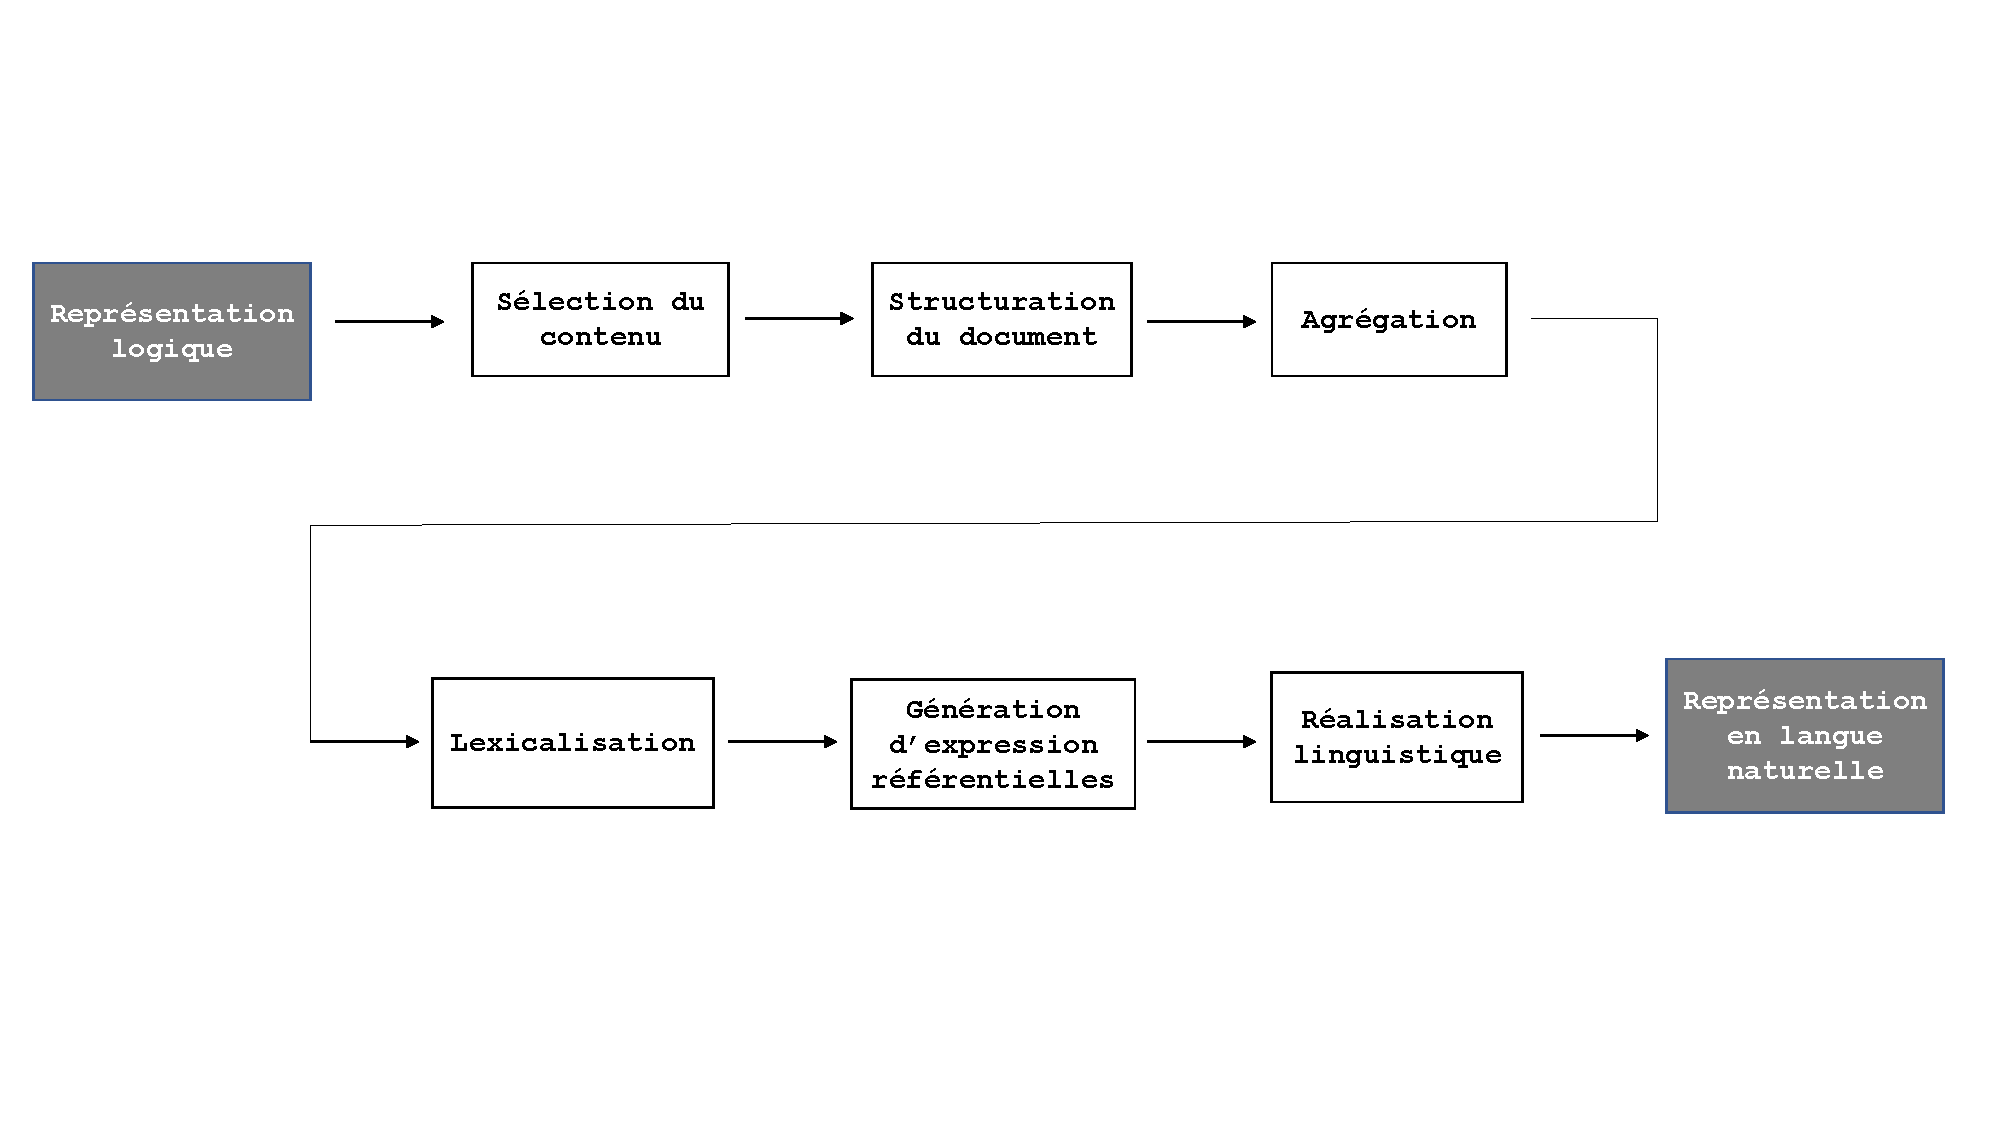
\includegraphics[width=1\textwidth, trim = {0cm 0cm 0cm 0cm},clip]{ch2/figs/pipeline.pdf}
	\caption{Pipeline classique, tiré de \citep{ReiterBuildingNaturalLanguage2000}}
	\label{fig:Pipeline}
\end{figure}

Un système de \ac{GAT} doit départir les informations qui seront exprimées dans le texte de celles qui n'y seront pas. Il s'agit donc de déterminer ce qui est pertinent dans les données brutes. Par exemple, si on souhaite générer le compte rendu d'un match de soccer, on ne voudrait probablement pas mentionner toutes les passes et toutes les fautes commises durant ce match, même si ces informations figurent dans les données de base. La \textbf{sélection du contenu} dépend aussi beaucoup du public à qui le texte est adressé et de l'objectif du texte: on ne présente pas la même information à un expert et à un novice. Dans le cas d'un compte rendu sportif, par exemple, on pourrait vouloir adapter le texte en fonction de l'équipe préférée du lecteur.

Ensuite, on crée \textbf{le plan du texte} à générer. Il s'agit de décider dans quel ordre présenter les informations sélectionnées. Cette étape est une représentation ordonnée et structurée du message à transmettre. Reprenons l'exemple du soccer. En fonctions des données choisies, le texte devra débuter par les informations générales liées au match (où et quand le match s'est déroulé), suivi du nom des équipes qui s'opposaient, de qui a gagné, puis des faits saillants du match.

\textbf{L'agrégation} est l'étape où on combine des messages en une seule phrase afin de rendre le texte plus fluide et agréable à lire. Les messages sélectionnés dans le plan (structuration du document) n'ont pas à être exprimé dans des phrases individuelles si on est capable de les combiner \citep{ChengCapturingInteractionAggregation2000}. Bref, cette étape sert à éviter la redondance et un style trop télégraphique.

La \textbf{lexicalisation} est l'étape où l'on traduit les données non-linguistiques en langue naturelle. Il s'agit de choisir les lexèmes qui seront utilisés pour transmettre le message voulu. Comme il existe naturellement plusieurs manières de rendre une même idée en mots, cette tâche peut devenir assez complexe si on veut que le système tienne compte des subtilités de la langue. La sélection des lexies peut ainsi se faire à divers niveaux d'abstraction. Un niveau plus abstrait requière plus de travail et est plus complexe à mettre en place. Toutefois, il génère plus de possiblités au moment de la réalisation. \cite{ElhadadFloatingConstraintsLexical1997} prônaient une approche en faveur de la lexicalisation profonde. Par exemple, un système de \ac{GAT} permettant une lexicalisation profonde pourrait générer les paraphrases suivantes: \form{Paul marque un but spectaculaire pendant la deuxième période} et \form{Paul réussi un but à couper le souffle lors de la seconde période}.

\textbf{La génération d'expressions référentielles} est très similaire à la lexicalisation car on choisit comment se réaliseront certaines entités. Le but est de s'assurer que le lecteur puisse distinguer correctement chaque entité. Pour cela, il faut trouver la meilleure façon de référer à une entité. Pour ces raisons, on l'appelle souvent \scare{l'étape discriminatoire}. Continuons avec l'exemple du soccer. Cette étape du processus nous permet de référer à une même joueur de diverses manières dans le texte. Par exemple: l'attaquant, la jeune recrue, Joe McCain, McCain, Little-Joe, le récipiendaire du prix McKenna, etc.

La dernière étape est \textbf{la réalisation linguistique}. Lorsque tous les mots et les expressions référentielles ont été choisis, on peut réaliser le texte final. Cette tâche implique l'application de traits morpho-syntaxiques aux lexèmes et la linéarisation des structures. Elle inclut aussi l'insertion des mots fonctionnels (auxiliaires, déterminants,etc.) et la ponctuation. Cette étape du processus nous intéresse particulièrement, donc nous élaborerons sur celle-ci.



%%%%%%%%%%%%%%%%%%%%%%%%%%%%%%%%%%%%%%%%%%%%%%%%%%%%%%%
% --------- R É A L I S A T I O N   ---------
%%%%%%%%%%%%%%%%%%%%%%%%%%%%%%%%%%%%%%%%%%%%%%%%%%%%%%%


\section{Réalisation}

Puisque nous avons maintenant traité du processus global de \ac{GAT} et des différentes méthodes de réalisation, nous pouvons entrer dans les détails de la tâche qu'est la réalisation linguistique, dans laquelle s'insère notre travail.

Tel qu'explicité à la figure~\ref{fig:Pipeline}, la réalisation est la dernière étape dans le processus de \ac{GAT}. Toutefois, pour beaucoup de chercheurs, elle ne représente pas uniquement les tâches décrites précédemment. Il règne en effet un certain flou autour de ce qui constitue la réalisation. Pour certains, elle correspond exactement à la description de la réalisation que nous fournissons en \ref{ppc}. On appellera cela la réalisation de surface, puisque la réalisation se fait à partir d'un input beaucoup plus près du texte (des structures syntaxiques lexicalisées). Pour d'autres, la réalisation se fait à partir de données plus abstraites, en amont de la lexicalisation. Ce type de réalisation plus profonde prend généralement en input des structures pré-syntaxiques. On les appellera des réalisateurs profonds. Dans ces systèmes, les informations lexicales et grammaticales seront encodées dans des dictionnaires et des grammaires plus complexes permettant de traiter l'interface sémantique-syntaxe. Finalement, ces systèmes profonds sont généralement liés à une théorie linguistique leur permettant de modéliser le langage et de l'encoder dans un système informatique.

\subsection{Types d'approches}

Il existe traditionnellement trois types d'approches pour la réalisation.

Nous nommerons d'abord, l'\textbf{approche à base de patrons}. Elle est généralement utilisée pour produire du texte dans des domaines spécifiques comme la météo ou les sports. Cette approche réduit la variation linguistique à un minimum puisque chaque réalisation de texte se fait à partir d'un moule fixe \citep{mcroy_channarukul_ali_2003}. Les phrases en \ref{template}, provenant de l'article de \cite{gatt18}, démontrent comment de tels patrons s'utilisent.

\ex. \label{template}
	\a.\$player scored for \$team in the \$minute minute. \label{a.}
	\b. Ivan Rakitic scored for Barcelona in the 4th minute.

En \ref{a.}, le patron contient trois variables, marquées par les \$. Celles-ci peuvent être respectivement comblées par un nom de joueur, suivi d'un nom d'équipe et d'une indication temporelle. L'avantage de cette approche est qu'on peut prévoir exactement ce qui sera généré et on diminue, par le fait même, les risques d'erreurs. L'inconvénient est que cette approche est très rigide et laisse place à quasi aucune paraphrase. Cependant, les réalisateurs à base de patrons peuvent être complémentés par des règles de grammaire, ce qui les rend plus flexibles. Toutefois, puisqu'ils sont codés à la main, ces sytèmes ont l'inconvénient d'être coûteux à développer. \cite{gatt18} soulignent qu'ils peuvent aussi être combinés à de l'apprentissage machine pour automatiser l'écriture des patrons, ce qui rend la tâche moins coûteuse. D'ailleurs, la combinaison d'approches est une démonstration de l'affaissement des frontières (création de systèmes hybrides) entre les méthodes traditionnelles de réalisation.

Ensuite, il y a l'approche \textbf{basée sur des règles grammaticales}. Celles-ci s'emploient autant dans les domaines spécifiques (météo, sport, etc.) que les domaines généraux (conversation libre). Ces systèmes de réalisation se prêtent bien à la langue courante puisqu'ils sont conçus pour représenter le langage à travers des règles de grammaire. Cependant, les grammaires et les dictionnaires nécessaires au bon fonctionnement de cette approche sont codés manuellement, ce qui demande du temps et des ressources.

Finalement, il y a les \textbf{méthodes statistiques}. On peut les utiliser pour filtrer les sorties d'un système à l'aide d'un modèle probabiliste qui déterminera quel output est le meilleur candidat \citep{LangkildeForestbasedStatisticalSentence2000} (aussi appellée l'approche \emph{generate-and-filter}). On peut aussi développer un modèle probabiliste permettant à un système de \ac{GAT} d'apprendre automatiquement les règles nécessaires pour générer du texte \citep{WhiteMinimalDependencyLength2012}. Les méthodes statistiques diminuent considérablement la charge de travail manuelle \citep{LangkildeForestbasedStatisticalSentence2000}.

Considérant les approches que nous venons de présenter, une question surgit quant à la nécessité de continuer à développer des méthodes à base de règles lorsqu'on peut sauver du temps et employer des méthodes probabilistes. À ce sujet, \cite{BelzSystemBuildingCost2009} se sont demandé si le temps gagné en automatisant la réalisation se faisait au détriment de la qualité et si c'était le cas, à quel point. Leur évaluation consistait à tester les deux méthodes en leur demandant de faire la même tâche. Ils ont ainsi considérer la qualité des textes via une évaluation humaine, puis une évaluation métrique faite automatiquement. Suite à l'analyse, ils nous expliquent que les évaluations humaines pointaient en faveur des systèmes à base de règles et que certaines évaluations métriques surévaluaient le système statistique et sous-évaluaient le système à base de règles.

Reiter s'est aussi penché sur la question et en a fait un survol dans un article tiré de son blog.\footnote{\url{https://ehudreiter.com/2016/12/12/nlg-and-ml/}, 12-03-18} Selon lui, même si les systèmes d'apprentissage automatique produisent généralement de bons textes, ils génèrent occasionnellement des bizarreries. Ce comportement n'est pas approprié dans des domaines professionnels où des utilisateurs comptent sur la qualité des textes, entre autre, car ils prendront potentiellement des décisions en fonction des textes générés. De plus, les systèmes basés sur des méthodes statistiques ont souvent plus de difficulté à corriger les incongruités. En revanche, les systèmes à base de règles permettent de cerner les problème avec plus de facilité et de les corriger. Cependant, Reiter termine son blog en soulignant que la \ac{GAT} a aussi beaucoup à gagner de l'emploi des méthodes statistiques. Il suggère qu'on se serve d'elles pour automatiser des étapes du processus de réalisation (à base de règles).

%%%%%%%%%%%%%%%%%%%%%%%%%%%%%%%%%%%%%%%%%%%%%%%%%%%%%%%
% --------- R É A L I S A T E U R   S U R F A C E ---
%%%%%%%%%%%%%%%%%%%%%%%%%%%%%%%%%%%%%%%%%%%%%%%%%%%%%%%

\subsection{Réalisateurs de surface}

Dans cette section, nous présenterons trois réalisateurs de surface connus: SimpleNLG, JSrealB et RealPro.

\subsubsection{SimpleNLG}
SimpleNLG \citep{GattSimpleNLGRealisationEngine2009} est un réalisateur de surface pour l'anglais écrit en java. Le texte est réalisé à partir d'une structure syntaxique déjà lexicalisée encodée en \emph{XML}. Par la suite, le réalisateur effectue les opérations morphologiques nécessaires (flexion, dérivation, ajout d'auxiliaires, gestion de l'accord) tout en linéarisant le texte.

Puisqu'il s'agit d'un réalisateur à base de règles, SimpleNLG est doté d'une grammaire et d'un dictionnaire. Ce dernier encode les propriétés syntaxiques et morphologiques des unités lexicales. Puis, le module grammatical contient des règles permettant le passage de la syntaxe à la morphologie.

SimpleNLG sépare son processus de réalisation en quatre étapes. Premièrement, les lexèmes compris dans la structure d'input sont mis en correspondance avec leurs entrées de dictionnaire. Deuxièmement, on détermine les traits spécifiques des lexèmes. Troisièmement, on combine les lexèmes en créant des syntagmes de plus en plus larges, jusqu'à ce que l'entièreté de la phrase forme un syntagme phrastique. Finalement, les règles morphologiques sont appliquées et les lexèmes sont accordés afin d'obtenir les formes fléchies.

SimpleNLG a également été adapté à d'autres langues, dont l'espagnol \citep{RamosSotoAdaptingSimpleNLGSpanish2017}, l'italien \citep{MazzeiSimpleNLGITadaptingSimpleNLG2016}, le français \citep{VaudryAdaptingSimpleNLGBilingual2013}, le portugais \citep{deOliveiraAdaptingSimpleNLGBrazilian2014} et l'allemand \citep{BollmannAdaptingSimpleNLGGerman2011}.

La figure~\ref{simplenlg} illustre l'input nécessaire permettant de réaliser la phrase \form{Refactoring is needed}. Elle provient du GitHub de SimpleNLG.\footnote{\url{https://github.com/simplenlg/simplenlg/blob/master/docs/XMLRepresentationOfTextSpecifications.pdf}}

\begin{figure}[htb]
 \caption{Structure d'input permettant de réaliser \form{Refactoring is needed} dans SimpleNLG}
 \label{simplenlg}
\begin{lstlisting}[language=Xml]
<Document>
  <child xsi:type="SPhraseSpec">
    <subj xsi:type="VPPhraseSpec" FORM="PRESENT_PARTICIPLE">
      <head cat="VERB">
        <base>refactor</base>
      </head>
    </subj>
    <vp xsi:type="VPPhraseSpec" TENSE="PRESENT" >
      <head cat="VERB">
        <base>be</base>
      </head>
      <compl xsi:type="VPPhraseSpec" FORM="PAST_PARTICIPLE">
        <head cat="VERB">
          <base>need</base>
        </head>
      </compl>
    </vp>
  </child>
</Document>
\end{lstlisting}
\end{figure}

\subsubsection{JSrealB}
JSrealB (pour \emph{JavaScript Realiser Bilingual}) \citep{DBLP:conf/enlg/MolinsL15} est conçu pour les programmeurs web, car il génère des expressions et phrases bien formées qui peuvent être formattées en \emph{HTML} pour ensuite être utilisées dans un fureteur. Toutefois, JSrealB peut aussi s'employer seul à des fins purement linguistiques.

Pour générer du texte, ce réalisateur prend en input des structures syntaxiques lexicalisées. Dans ce système, la construction de la phrase découle de l'application de règles syntaxiques et morphologiques déclenchées par les lexèmes. De plus, JSrealB fonctionne aussi avec un dictionnaire et une grammaire. Son dictionnaire définit la catégorie des lexèmes qui le peuple et leurs traits lexicaux (genre, nombre, irrégularités, etc.), pui sa grammaire contient des règles morpho-syntaxiques qui lui permettent de faire l'accord entre les constituants. Finalement, il existe aussi une version bilingue de JSrealB \citep{MolinsJSrealBBilingualText2015} qui incorpore le français et l'anglais. L'input qu'illustre la figure~\ref{jsreal} permet au réalisateur de générer la phrase: \form{The cat sat on the coach}. Cet exemple est tiré du GitHub de JSrealB.\footnote{\url{https://github.com/rali-udem/JSrealB}}

\begin{figure}[htb]
\caption{Structure d'input réalisant \form{The cat sat on the coach} dans JSrealB}
\label{jsreal}
\begin{lstlisting}[language=mate]
JSrealLoader({
        language: "en",
        lexiconUrl: URL.lexicon.en,
        ruleUrl: URL.rule.en,
        featureUrl: URL.feature
    }, function() {
    QUnit.test( "Sentence EN", function( assert ) {
        assert.equal(
            S(
                NP(D("the"), N("cat")),
                VP(V("sit"), PP(P("on"), NP(D("the"), N("coach")))).t("ps")
            )
\end{lstlisting}
\end{figure}
		
\subsubsection{RealPro}
RealPro \citep{LavoieFastPortableRealizer1997} est implémenté en \emph{C++} et c'est le plus profond des réalisateurs de surface préséntés ici. Il prend en input des arbres de dépendances, ce qui le distingue des deux autres systèmes qui utilisent des arbres de constituants \citep{DBLP:conf/enlg/MolinsL15,GattSimpleNLGRealisationEngine2009}. Rapidement, un arbre de dépendance est un arbre non-linéarisé dont les arcs et les n\oe{}uds (des lexèmes) sont étiquetés. On appelle ça un arbre syntaxique car les branches liant les n\oe{}uds entre eux correspondent à des relations syntaxiques. Seuls les mots sémantiquement pleins figurent dans l'input (cela exclut les déterminants, prépositions, etc.).

Cette architecture est basée sur la \ac{TST} \citep{melcuk1988}, une théorie linguistique qui a fait ses preuves en \ac{GAT} \citep{iordanskaja88,LavoieFastPortableRealizer1997,WannerMARQUISGENERATIONUSERTAILORED2010,MilledemoFORGePompeu2017,Vicentegeneracionlenguajenatural2015}.

En bref, il s'agit d'une théorie qui divise le langage en quatre niveaux de représentations majeurs: sémantique, syntaxique (profonde et de surface), morphologique (profonde et de surface), phonologique (profonde et de surface) -- ce dernier étant court-circuité pour la génération de texte écrit. Pour plus de détails concernant les arbres de dépendances et la \ac{TST}, voir le chapitre~\ref{chapgendr}.

RealPro \citep{LavoieFastPortableRealizer1997} a deux grammaires qui permettent successivement de passer d'une représentation profonde à une représentation de surface, puis de celle-ci à une linéarisation morphologique de l'input. Pour effectuer toutes les transitions, le système fait aussi appel à un dictionnaire qui encode les propriétés lexicales et morphosyntaxiques des unité. Le graphique \ref{fig:RealPro} illustre l'interaction de ces deux ressources pour réaliser du texte.

\begin{figure}[htb]
	\centering
	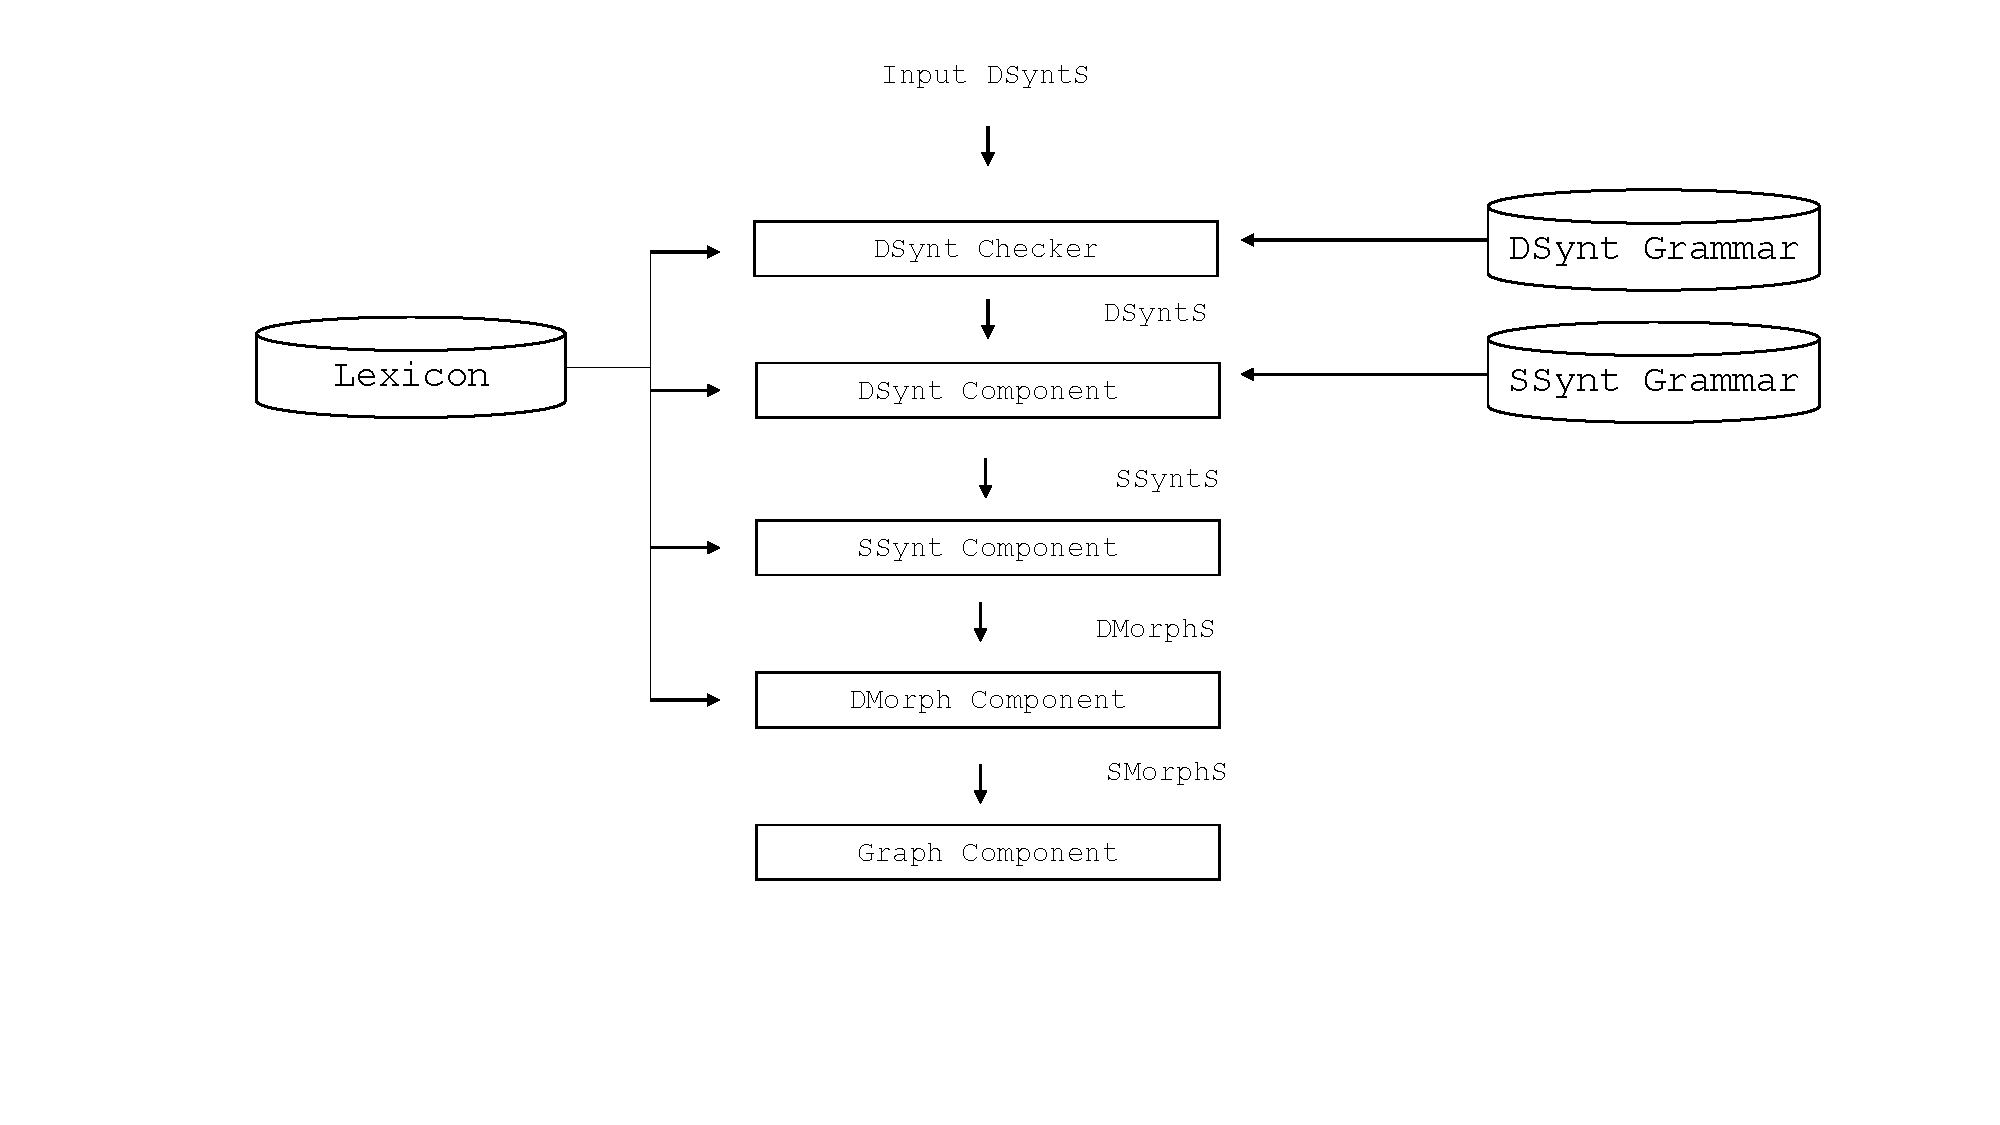
\includegraphics[width=1\textwidth, trim = {0cm 0cm 0cm 0cm},clip]{ch2/figs/realpro.pdf}
	\caption{Modules dictionnairiques et grammaticaux de RealPro}
	\label{fig:RealPro}
\end{figure}

La figure~\ref{lst:realpro} illustre un arbre de dépendance (l'input) représentant la phrase \form{March had some rain days}; elle provient de \cite{ReiterBuildingNaturalLanguage2000}.

\begin{figure}[htb]
\caption{Input de la phrase \form{March had some rain days} dans RealPro}
\label{lst:realpro}
\begin{lstlisting}[language=mate]
HAVE1 [tense:past]
(I March [class:proper-noun]
II day [class:common-noun numberpl]
(ATTR rainy [class:adjective]))
\end{lstlisting}
\end{figure}

%%%%%%%%%%%%%%%%%%%%%%%%%%%%%%%%%%%%%%%%%%%%%%%%%%%%%%%
% --------- R É A L I S A T E U R    P R O F O N D  ---
%%%%%%%%%%%%%%%%%%%%%%%%%%%%%%%%%%%%%%%%%%%%%%%%%%%%%%%

\subsection{Réalisateurs profonds}

Les réalisateurs profonds prennent généralement en input des structures plus abstraites, ce qui permet de réaliser des phénomènes langagiers plus profonds. Comme les réalisateurs profonds incorporent généralement la lexicalisation, cela fait en sorte qu'un seul input produit souvent plusieurs outputs \citep{PolguerePourmodelestratifie1998}, autrement dit, ces systèmes ont un grand pouvoir paraphrastique. Dans le pipeline classique, comme nous l'avons vu à la section \ref{ppc}, la lexicalisation est opérée avant la réalisation. Cet ordre a pour conséquence que les inputs fournis au réalisateur sont déjà lexicalisés et cela restreint grandement les réalisations possibles (puisque les lexèmes incorporent des propriétés de combinaitoires bien précises autours desquelles la phrase doit s'articuler). 

Dans cette section, nous présenterons les réalisateurs profonds suivants: KPML, SURGE, FORGe et MARQUIS.

\subsubsection{KPML}
KMPL \citep{BatemanEnablingTechnologyMultilingual1997} est un réalisateur multilingue issu du système PENMAN \citep{PenmanOverview}. La théorie linguistique sous-jacente à ce système est la \ac{SFG} \citep{MatthiessenSystemicfunctionalgrammar1997}, qui postule que les choix linguistiques sont déclenchés par l'exécution de fonctions grammaticales. D'un point de vue multilingue, les différentes langues issues de KPML partagent la majorité des fonctions grammaticales. Ces fonctions forment le c\oe{}ur du système, mais il existe aussi quelques fonctions propres à chaque langue pour réaliser les phénomènes linguistiques spécifiques à chacune.

La grammaire de ce système est implémentée à la manière d'un réseau orienté. Chaque intersection dans le réseau correspond à un choix grammatical à faire entre différents traits fonctionnels. Ces choix deviennent de plus en plus précis lorsqu'on avance dans le réseau. Ainsi, la forme de surface d'un input donné est la conséquence du parcours de ces réseaux.

Les informations comprises dans les inputs de ce système sont d'ordre sémantique et syntaxique. Ainsi, l'input de KPML est un \ac{SPL}, ce qui est une matrice d'attributs et de valeurs. La figure~\ref{kpml} illustre un \ac{SPL} et elle est issue de \cite{ReiterBuildingNaturalLanguage2000}.

\begin{figure}[htb]
\caption{SPL: input pour réaliser \form{March had some rainy days} dans KPML}
\label{kpml}
\begin{lstlisting}[language=mate]
(S1 \ generalized-possession
  :tense past 
	:domain (N1 \ time-interval
	            :lex march
							:determiner zero)
	:range (N2 \ time-interval
	           :number plural
						 :lex day
						 :determiner some
						 :property ascription
						 (A1 \ quality :lex rainy)))
\end{lstlisting}
\end{figure}

\subsubsection{SURGE}
SURGE, qui signifie \emph{Systemic Unification Realisation Grammar of English}, est une grammaire de l'anglais \citep{Elhadad98surge:a} qui est écrite en \ac{FUF}: une grammaire basée sur \acf{FUG} \citep{KayFunctionalUnificationGrammar1984}. \ac{FUF} est un langage de programmation créé pour construire des grammaires d'unification informatisées.

SURGE prend en input des arbres thématiques non linéarisés dont les n\oe{}uds sont des unités sémantiques pleines (donc ça exclut les prépositions,etc.). Ces arbres sont représentés comme des structures de traits encodés dans le formalisme \ac{FUF}. Ces structures de traits sont appellées des \ac{FD}. Il s'agit d'ensemble de paires d'attributs-valeurs qui peuvent être sucessivement enchâssées. Les entrées lexicales et leurs propriétés sont directement encodées dans les \ac{FD} ce qui fait en sorte que SURGE n'a pas besoin de dictionnaire. Chaque constituant se fait attribuer une catégorie syntaxique et c'est grâce à ces traits que la grammaire sait comment unifier la phrase.

Dans ce système, la grammaire est aussi décrite en termes de \ac{FD}. Ainsi, pour réaliser du texte, SURGE prend en entrée à la fois les \ac{FD} du sens de la phrase désirée et les \ac{FD} représentant les règles de grammaire du système afin d'unifier les structures. Le résultat est une structure d'entrée enrichie par des spécifications grammaticales (syntaxique et morphologique). Cela permet au réalisateur de passer à l'étape suivante qui est la linéarisation. SURGE applique ainsi les traits morphologiques en fonction des spécifications encodées lors de l'unification. L'output est une phrase anglaise exprimant le sens de la \ac{FD} en fonction des contraintes imposées par la grammaire.

Nous reprenons encore un exemple tiré de \cite{ReiterBuildingNaturalLanguage2000}: \form{March had some rainy days}.

\begin{figure}[htb]
 \caption{FD: input pour réaliser \form{March had some rainy days} dans SURGE}
 \label{surge}
\begin{lstlisting}[language=mate]
((cat clause)
 (proc ((type possessive)))
 (tense past)
 (partic ((possessor ((cat proper) head ((lex "March"))))
					(possessed ((cat common) head ((lex day)))
											(describer ((lex rainy)))
											(selective yes) (number plural)))))
\end{lstlisting}
\end{figure}

\subsubsection{MARQUIS}\label{sectionmarquis}
Comme RealPro, MARQUIS est basé sur la \ac{TST}, mais contrairement aux autres systèmes présentés ici, MARQUIS n'est pas qu'un réalisateur profond. Il s'agit d'un système de \ac{GAT} complet qui effectue toutes les étapes du processus de génération automatique de texte (voir \ref{ppc}). Cependant, nous ne nous intéresserons ici qu'à son module de réalisation profonde \citep{Lareau2007TowardsAG}. Pour plus d'informations concernant le pipeline complet de MARQUIS, voir \citep{WannerMARQUISGENERATIONUSERTAILORED2010,bohnet07}. 

Le but du projet MARQUIS était de générer, à partir de données brutes, des bulletins météorologiques multilingues sur la qualité de l'air. Ces bulletins sont produits en fonction de l'utilisateur. Autrement dit, ceux-ci se créent des profils avec leurs informations personelles et cela permet à MARQUIS de réaliser du texte en fonction de leur niveau de connaissance du domaine et de leurs besoins de santé. Le tout est fait à partir d'un input conceptuel partagé par toutes les langues traitées par MARQUIS (l'anglais, l'allemand, l'espagnol, le catalan, le portugais, le français, le finnois et le polonais). 

La figure~\ref{fig:marquis} illustre le processus de réalisation que MARQUIS entreprend pour générer du texte. On peut y voir que le système prend en input des graphes conceptuels et qu'il produit du texte. Pour arriver à la réalisation finale, le réalisateur prend la structure \#1 en input, puis il lui applique des règles pour qu'il en résulte la structure \#2. Celle-ci lui servira d'input au prochain niveau de représentation. Cette transduction est ainsi répétée jusqu'à ce que le système se rende au dernier niveau de représentation, le texte.

\begin{figure}[htb]
	\centering
	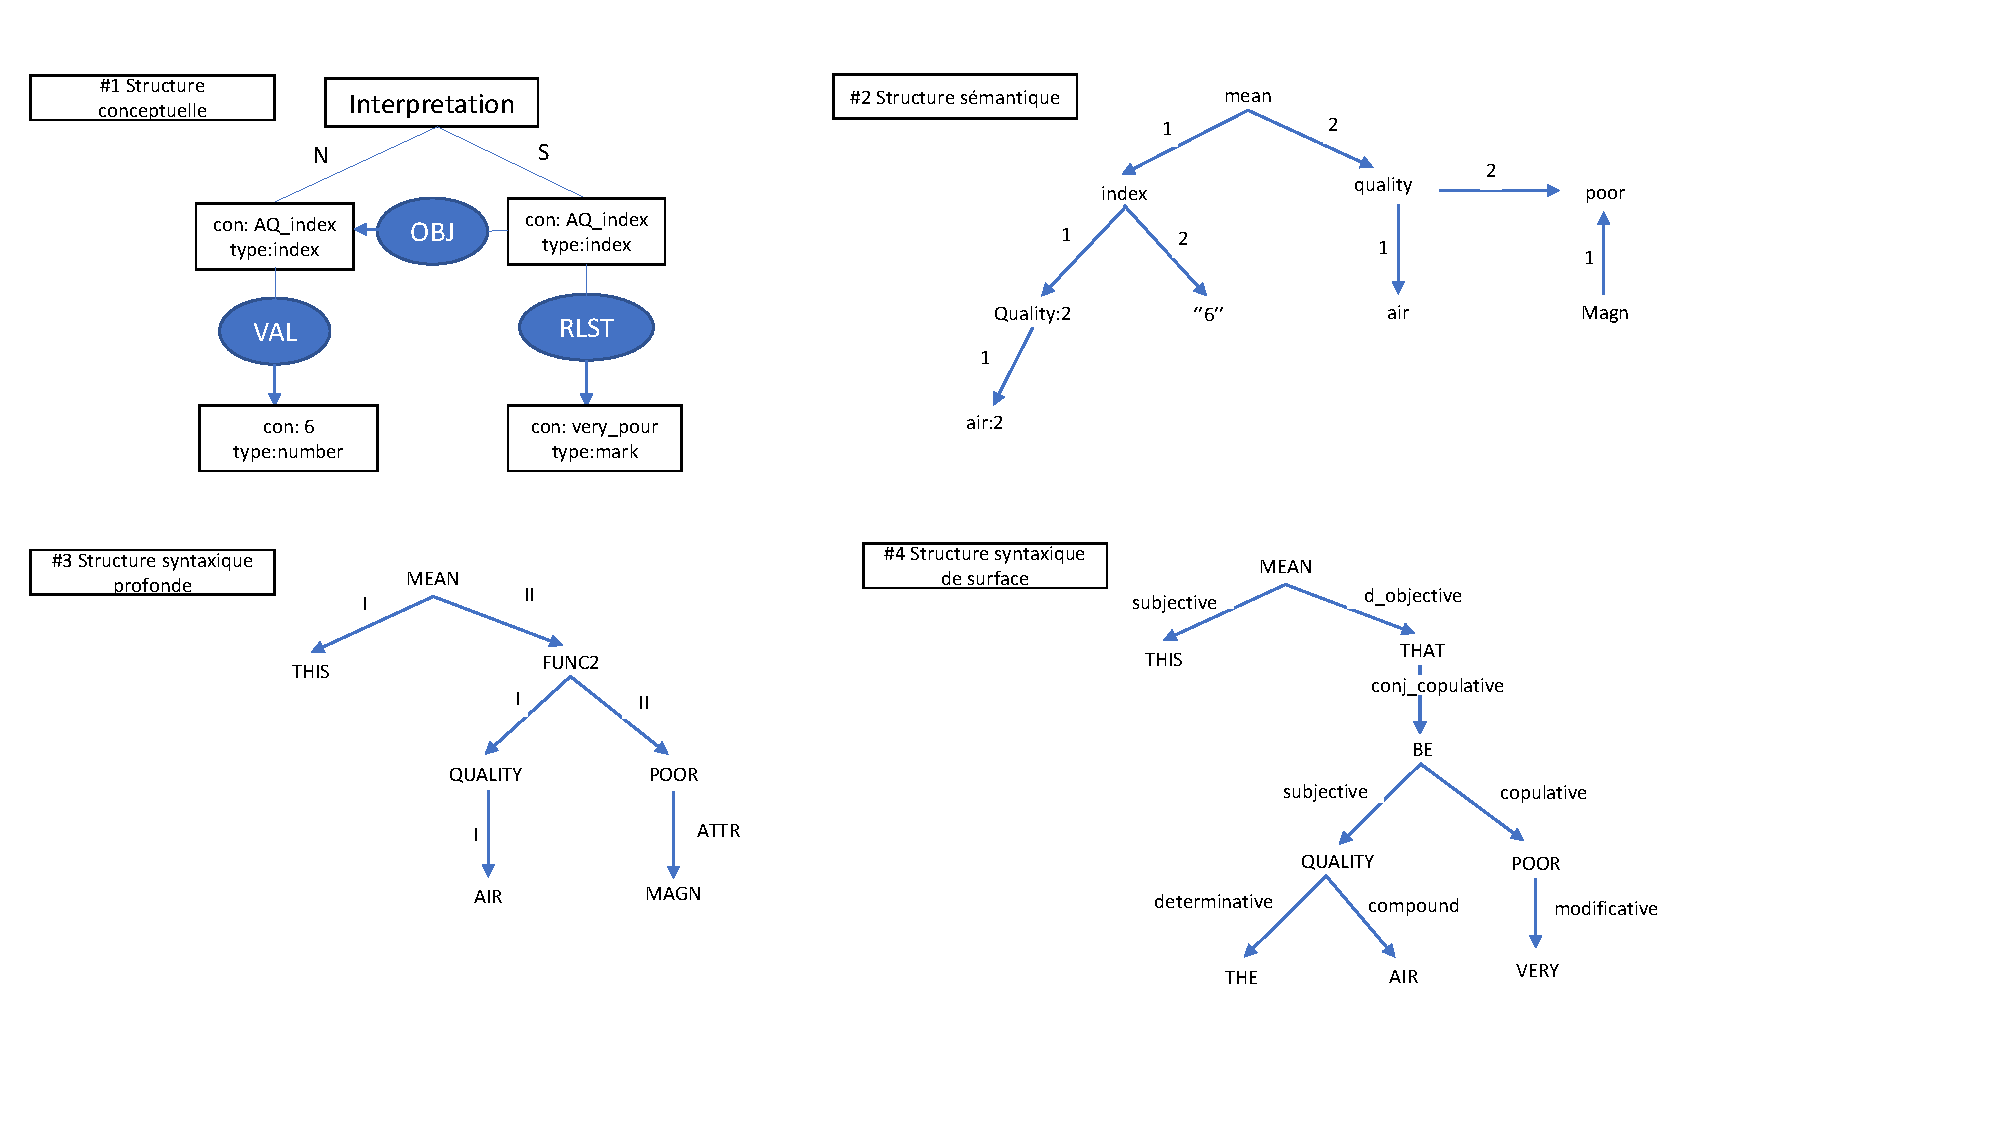
\includegraphics[width=1\textwidth, trim = {0cm 0cm 0cm 0cm},clip]{ch2/figs/marquis.pdf}
	\caption{Pipeline de MARQUIS \citep{WannerMARQUISGENERATIONUSERTAILORED2010}}
	\label{fig:marquis}
\end{figure}

Nous expliquerons brièvement ici les mécanismes qui permettent la transition d'une représentation à une autre (plus de détails suivront à la section \ref{sec:semsynt}). Il faut d'abord que le système analyse la structure conceptuelle à l'aide des règles de transduction qui permettent de passer de la représentation conceptuelle à la représentation sémantique. Le passage des unités conceptuelles aux unités sémantique se fait grâce aux informations encodées dans un dictionnaire à cet effet. Ensuite, après que la structure sémantique soit créée, MARQUIS la prend pour en dériver un arbre de dépendances syntaxique profond grâce aux règles de transduction de cette interface (sémantique-syntaxe). La mise en correspondance d'unités sémantiques et lexicales est opérée grâce au dictionnaire sémantique (\emph{semanticon}) et lexical (\emph{lexicon}) ainsi qu'au dictionnaire de fonctions lexicales. Finalement, les autres transitions de représentations sont assurées par des règles de transductions successives et les informations contenues dans le \emph{lexicon}. La figure~\ref{fig:reglesdict} présente ce mécanisme.

\begin{figure}[htb]
	\centering
	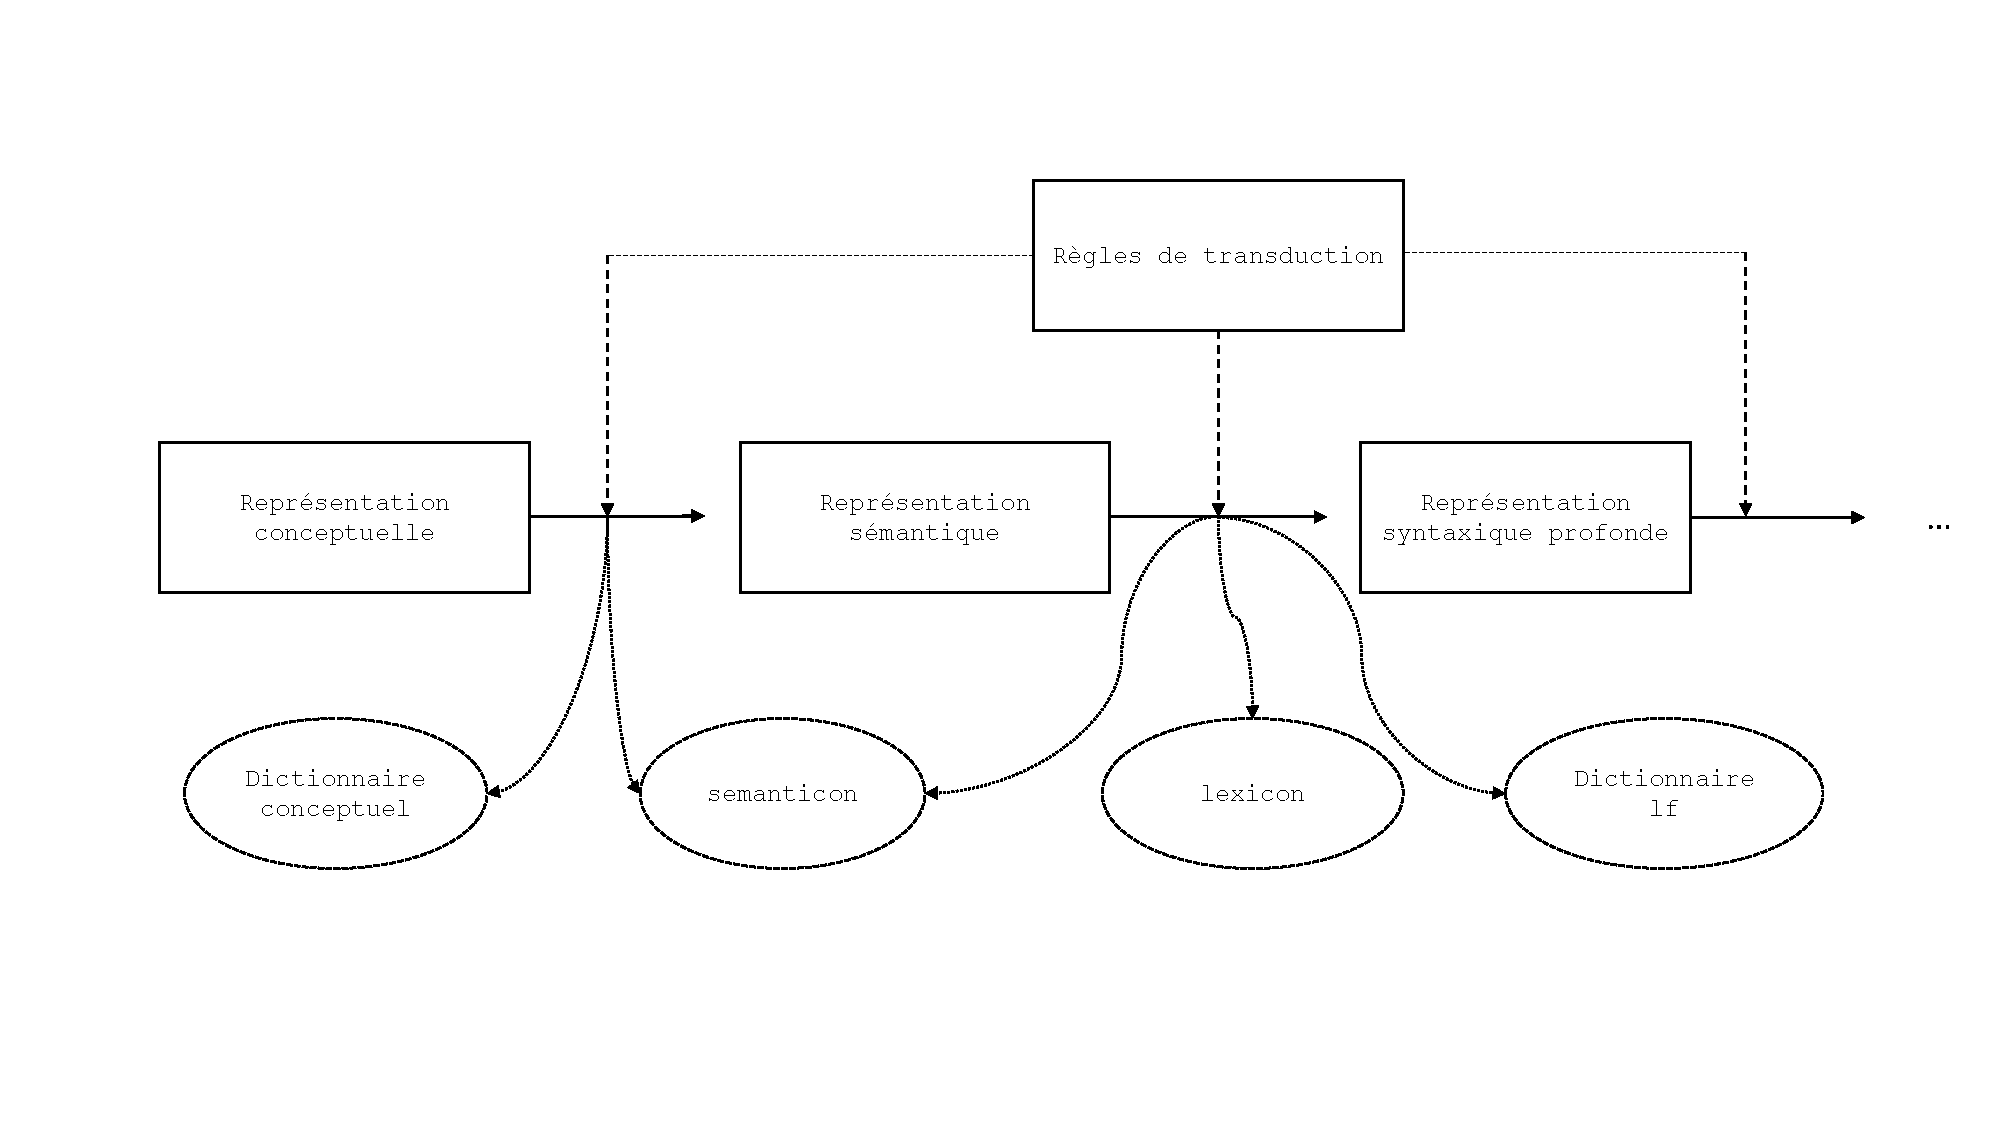
\includegraphics[width=1\textwidth, trim = {0cm 0cm 0cm 0cm},clip]{ch2/figs/module.pdf}
	\caption{Combinaison des règles et dictionnaires pour effectuer les transductions de graphes \citep{LambreyImplementationcollocationspour2017}}
	\label{fig:reglesdict}
\end{figure}

Pour mieux comprendre à quoi servent les dictionnaires mentionnés dans le paragraphe précédent, nous les décrirons rapidement. Le dictionnaire conceptuel comprend tous les concepts utiles à la génération des rapports sur la qualité de l'air et des termes du domaine général. Ce dictionnaire mappe les concepts aux unités sémantiques pour chaque langue traitée par le système. Le dictionnaire sémantique mappe les unités sémantiques aux lexies. Finalement, il nous faut un dictionnaire lexical qui contient toutes les unités lexicales avec leurs propriétés syntaxiques et morphologiques et leur combinatoire lexicale pour que le texte généré soit grammatical.

\subsubsection{FORGe}
FORGe est un transducteur de graphes qui génère du texte à l'aide de ressources lexicales dictionnairiques et grammaticales \citep{MilledemoFORGePompeu2017,DBLP:conf/semeval/MilleCBW17}. C'est un réalisateur profond qui a hérité de l'architecture de Marquis \citep{WannerMARQUISGENERATIONUSERTAILORED2010}. FORGe a été conçu pour l'anglais à la base, mais il se veut multilingue (espagnol, allemand, français et polonais sont en développement). C'est un réalisateur qui peut aisément générer du texte en différentes langues grâce à ses règles grammaticales, qui seront majoritairement partagées par toutes les langues.

La théorie linguistique sous-jacente à ce système est la \ac{TST} \citep{melcuk1988, mel2012semantics, PolgueretheorieSensTexte1998, kahane05a, Milicevic2007ASG} \footnote{Nous verrons plus en détail au chapitre \ref{chapgendr} comment cette théorie linguistique se prête à des transducteur de graphes.}.

FORGe prend en input des représentations sémantiques sous forme de graphes orientés acycliques représentant les relations prédicats-arguments entre des sémantèmes,ce qui correspond à la structure \#2 dans la figure~\ref{fig:marquis} de la section MARQUIS \ref{sectionmarquis}. Plus haut, nous avons vu que RealPro \citep{LavoieFastPortableRealizer1997} réalisait du texte en passant par la \ac{RSyntP} en traversant la syntaxe de surface, puis la morphologie pour que le tout soit linéarisé. FORGe fonctionne essentiellement sur les mêmes bases, mais son input est encore plus profond que la \ac{RSyntP}, il s'agit de la \ac{RSem}. Autrement dit, une représentation dépourvue de structure où les relations entre les n\oe{}uds ne sont que prédicats-arguments. Ainsi, la réalisation de texte dans FORGe se découpe en trois étapes: le transfert de la \ac{RSem} à la \ac{RSyntP}, suivi du transfert de la \ac{RSyntP} à la \ac{RSyntS}, et finalement de la \ac{RSyntS} au texte linéarisé et morphologisé. Le fonctionnement est donc très similaire à celui de RealPro, mais FORGe peut ainsi traiter beaucoup plus de phénomènes langagiers puisqu'il n'est pas contraint par les propriétés de combinatoire des unités lexicales dans sa structure d'input.

La première étape de réalisation est le passage de la sémantique à la syntaxe profonde qui est effectué via un algorithme récursif qu'on appelle \scare{\emph{top-down}}. Tel que nous le verrons dans le chapitre suivant à la section \ref{sec:arbo}, on rèfère à cet algorithme dans la \ac{TST} comme \textbf{l'arborisation}. En résumé, on crée un arbre syntaxique de dépendances à partir d'une \ac{RSem} qui précise un n\oe{}ud dominant. Celui-ci sera l'équivalent du \emph{top} (qu'on appelle la racine) qui se fait généralement imposé une partie du discours verbale. Cette restriction s'impose souvent, car on veut que le lexème qui consommera la racine soit un verbe, puisque ce sont eux qui contrôlent généralement la phrase. Une fois que la racine est lexicalisée, on peut désormais ajouter des branches qui font office de relation syntaxique entre la racine et les arguments qu'elle sélectionne. Les n\oe{}uds au bout de ces branches sont vides et contraints par le gouverneur afin que seuls les lexèmes respectant les contraintes soient lexicalisés. On dit que cet algorithme est récursif car ces opérations se répètent jusqu'à ce que l'arbre représente en syntaxe profonde la \ac{RSem} qu'on lui avait donné en entrée. Cette construction se fait sur les bases des dictionnaires et de la grammaire pour s'assurer que ce sera un arbre bien formé.

Ensuite, la seconde étape est le passage de la \ac{RSyntP} à la \ac{RSyntS}. Cela correspond à l'étape où on introduit les mots fonctionnels (prépositions, auxiliaires, déterminants) et les relations de surface (sujet, objet direct, etc.) dans l'arbre de dépendance créé à l'étape précédente. C'est là que FORGe se démarque de MARQUIS. L'héritier de ce dernier possède un dictionnaire de verbes qui explicite les comportements syntaxiques de ceux-ci. Cela permet de rendre compte de la richesse linguistique des verbes et de générer encore plus de paraphrases puisque c'est cette partie du discours qui contrôle généralement la construction d'un arbre. Nous reviendrons à cette problématique dans la section \ref{sec:gp} au chapitre \ref{chapgendr}.
                                                                                                                     
Finalement, la dernière étape pour achever la réalisation dans FORGe consiste à linéariser la structure syntaxique de surface et à appliquer les règles morpho-syntaxiques aux lexèmes pour produire le texte final.

En conclusion, MARQUIS et FORGe partent de niveaux d'abstraction plus profonds que les autres systèmes présentés. Cela leur permet d'être plus flexibles dans leurs réalisations. C'est pourquoi nous travaillerons avec un réalisateur profond très similaire à ces deux réalisateurs. Comme FORGe, nous utiliserons aussi un système basé sur MARQUIS, le système GenDR \citep{lambrey15,LambreyImplementationcollocationspour2017,lareau18}, que le chapitre suivant décrira en détail.
